\documentclass[./dissertation.tex]{subfiles}
\chapter{Technical Analysis}
\label{PICORV32_anal}
In this chapter, a description of one of the LHC detectors at CERN is given, as to give a better understanding of the environment and setting in which the SoC is planned to function. Following this, a theoretical outline is given for radiation and its effects on CMOS electronics and how this can be mitigated by design choice. Following this, an method for extensive verification of individual block and system verification is presented. After this a description of the steps of physical implementation is given and finally the choice of CPU for the SoC is made, which is accompanied by a description of the state of the system at the beginning of the author's internship and the future plans for it.

\section{LHC Detectors at CERN}
\label{detectors}
There is a vast complex network of different accelerators and different detectors at CERN. The highest energy endpoint in this network is the LHC. The LHC is a \SI{27}{km} counter-rotating accelerator. Using superconducting magnets, it is capable of accelerating protons up to a peak energy level of \SI{7}{TeV}, which results in a peak collision energy of \SI{14}{TeV}. To reach these energy levels, a network of several accelerators is used to initially accelerate the protons to \SI{450}{GeV} before they are injected into the LHC. In the LHC the beams collide with a bunch spacing of \SI{25}{ns} corresponding to a frequency of \SI{40}{MHz} and is called the bunch-crossing (BX) rate. The entire network can be seen in figure \ref{fig:accelerator_network_cern}. More details can be read in the article: LHC Machine \cite{LHCmachine}.

\begin{figure}[H]
    \centering
    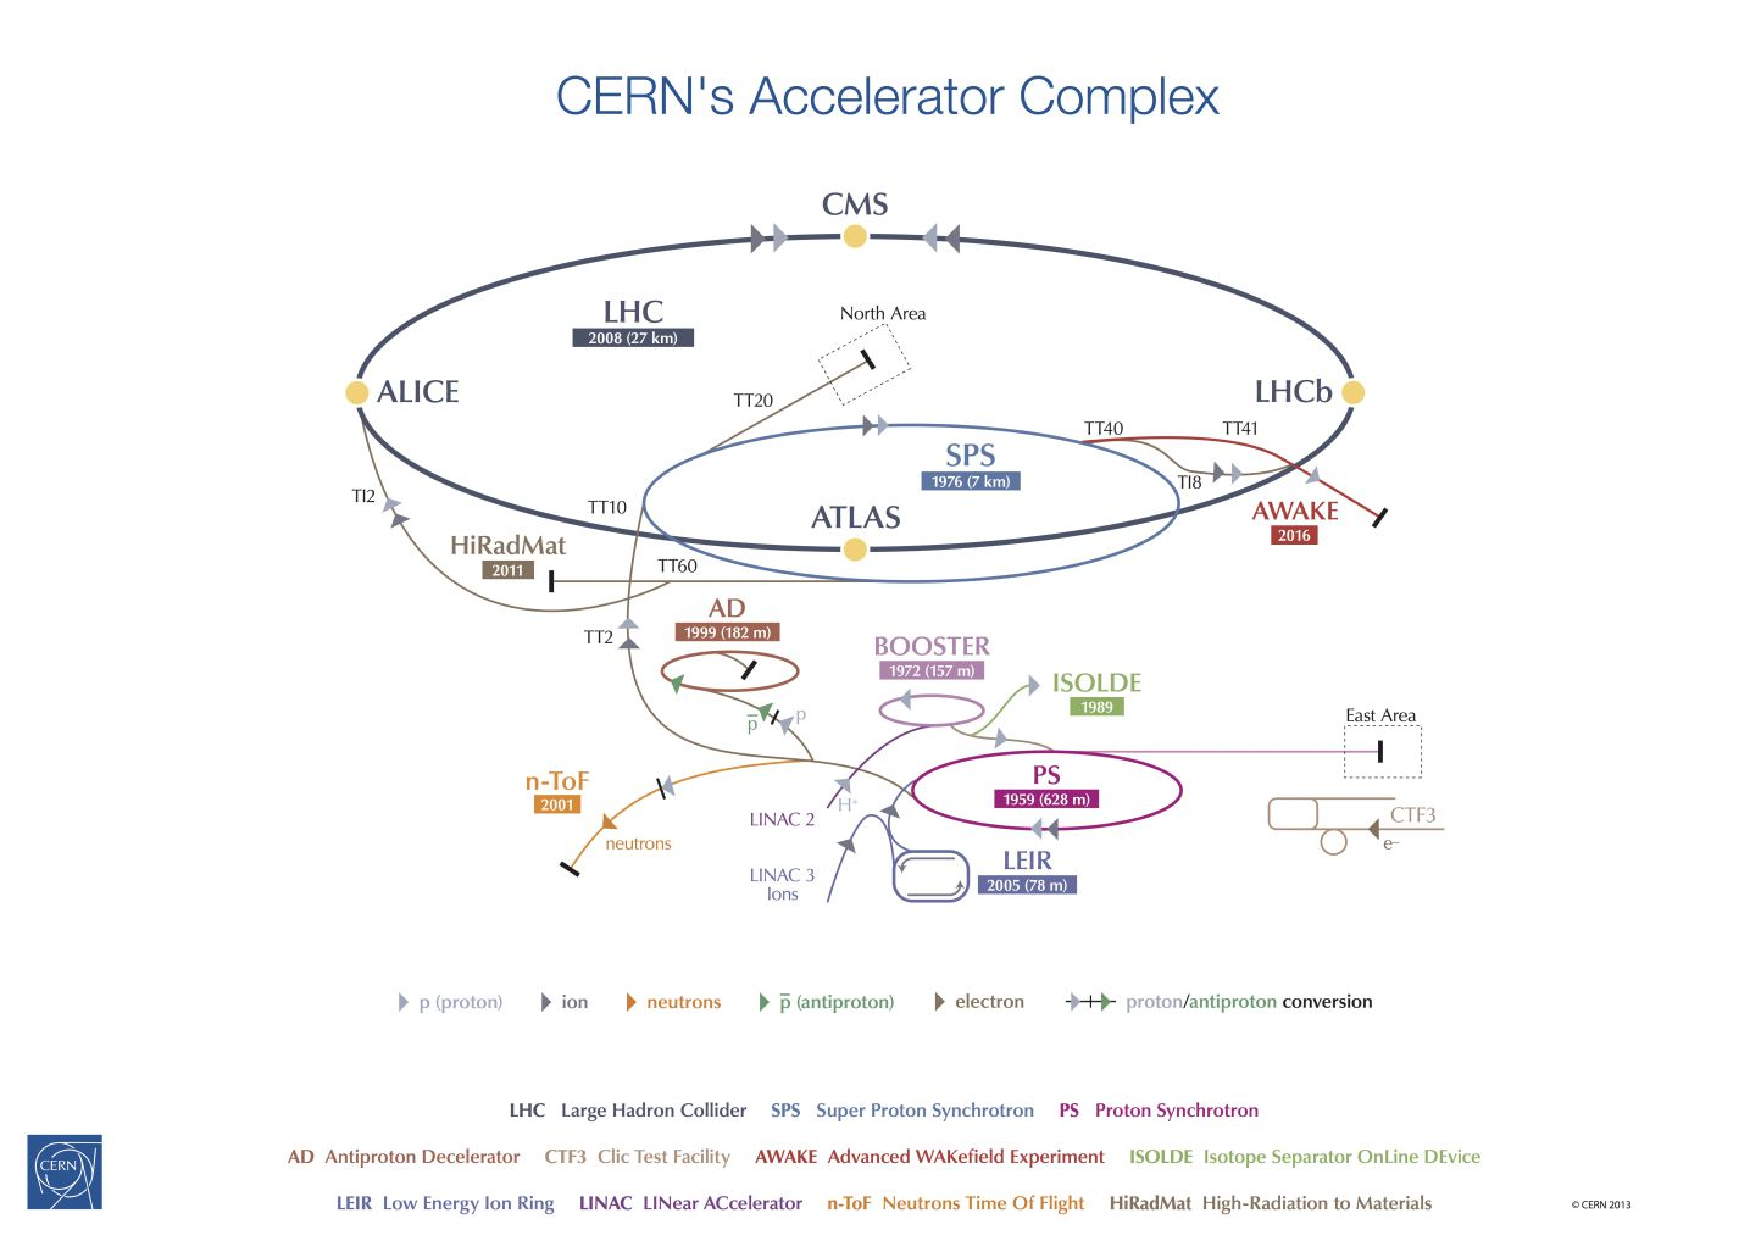
\includegraphics[width=\linewidth]{subfiles/imgs/acceleratorNetworkCERN.pdf}
    \caption{Shows the complete network of used accelerators at CERN (Courtesy of \cite{Haffner:1621894}).}
    \label{fig:accelerator_network_cern}
\end{figure}

There are four detectors placed on the LHC ring. These are A Large Ion Collider Experiment (ALICE), Compact Muon Solenoid (CMS), Large Hadron Collider Beauty (LCHb) and A Toroidal LHC ApparatuS (ATLAS). These 4 experiments can be split into 3 categories. CMS and ATLAS are general-purpose onion detectors, which means they try to detect all particles created by the collision. These two are built in different ways by different independent teams such that they can be used to verify the results of each other. ALICE is an experiment focused on the collision of heavier ions, e.g. lead ions. LCHb is a detector focused on only detecting the particles created by collision, which moves in the beam direction. This makes it possible for them to make a specialized detector better suited for detecting the particles in that specific direction. A majority of the particles created in this experiment are related to the beauty quark, which gives reason to its name. A detailed description of CMS, one of the general-purpose experiments, will now be given. This will lay the foundation for understanding the environment in which the electonics are expected to survie and give a reasoning to some of the design choices made later.

The CMS sits at one of the four collision points in LHC. Figure \ref{fig:cms_layout} shows the layout of the CMS detector. The particles generated in the collisions propagate radially, traversing the silicon tracker. The silicon tracker measures the particle trajectory and transverse momentum $p_T$. The silicon tracker is composed of an all-silicon pixel and strip tracker \cite{collaboration2008cms}. Next are the electromagnetic calorimeter (ECAL) and the hadron calorimeter (HCAL). The calorimeters enable the evaluation of the particle energy. The ECAL uses lead tungstate scintillating crystals for this purpose \cite{collaboration2008cms}. Scintillating crystals emit photons when ionizing particles pass through them. The light is then detected by silicon avalanche photodiodes (APD) in the barrel region and vacuum phototriodes (VPT) in the endcap region. The APD makes use of the avalanche effect, where a single charged particle can knock multiple electrons out of their bond and thereby amplifying their electrical signature. The VPTs are single amplification stage photomultipliers. They have a photocathode at ground potential, a single dynode biased at \SI{+600}{V}, and an anode biased at \SI{+800}{V}. VPTs operate by a photon hitting the cathode which releases electrons. The released photoelectrons are accelerated towards the dynode, where each photoelectron releases multiple new photoelectrons. These are then accelerated towards the anode as it is at a higher potential. The anode then produces an amplified current.     

After the ECAL, the particles enter a brass/scintillator HCAL \cite{collaboration2008cms}. Here the scintillation light is collected by wavelength-shifting (WLS) fibers embedded in the scintillator tiles. The WLS fibers emit multiple low-energy photons for each high-energy photon strike. This light is channeled to photodiodes which amplify the signal. The aforementioned components are encapsulated by a \SI{3.8}{T} superconducting solenoid. Outside the superconducting solenoid, the iron return yoke with muon chambers is placed. The iron return yoke confines the magnetic field and stops all remaining particles except for muons and neutrinos. The muon system has 3 functions: muon identification, momentum measurement, and triggering. In the barrel, region detection is done using drift tubes while in the end-cap region it is done using cathode strip chambers. Both of these systems are completed by a dedicated trigger system of resistive plate chambers.

In total, the CMS detector has a diameter of \SI{15}{m}, a length of \SI{28.7}{m}, and weighs $14 \cdot 10^6$ \si{kg}.

\begin{figure}[H]
    \centering
    \includegraphics[width=\linewidth]{subfiles/imgs/cms_layout.png}
    \caption{Shows the layout of the CMS detector \cite{CMSdetector}.}
    \label{fig:cms_layout}
\end{figure}

The CMS is capable of detecting a wide range of particles using the collection of the data from each of its components. Different particles will follow a different path through the detector based on their charge, momentum, and trajectory. In figure \ref{fig:particles_in_cms} a path of the common particles can be seen. The superconducting solenoid enables the estimation of the charge and momentum of a particle. The charge can be determined by the bend direction of the trajectory because positively charged particles will bend opposite to negatively charged particles and neutral particles will not bend at all. The momentum can then be estimated by the degree of bending as faster-moving particles will bend less than slow-moving particles. 

\begin{figure}[H]
    \centering
    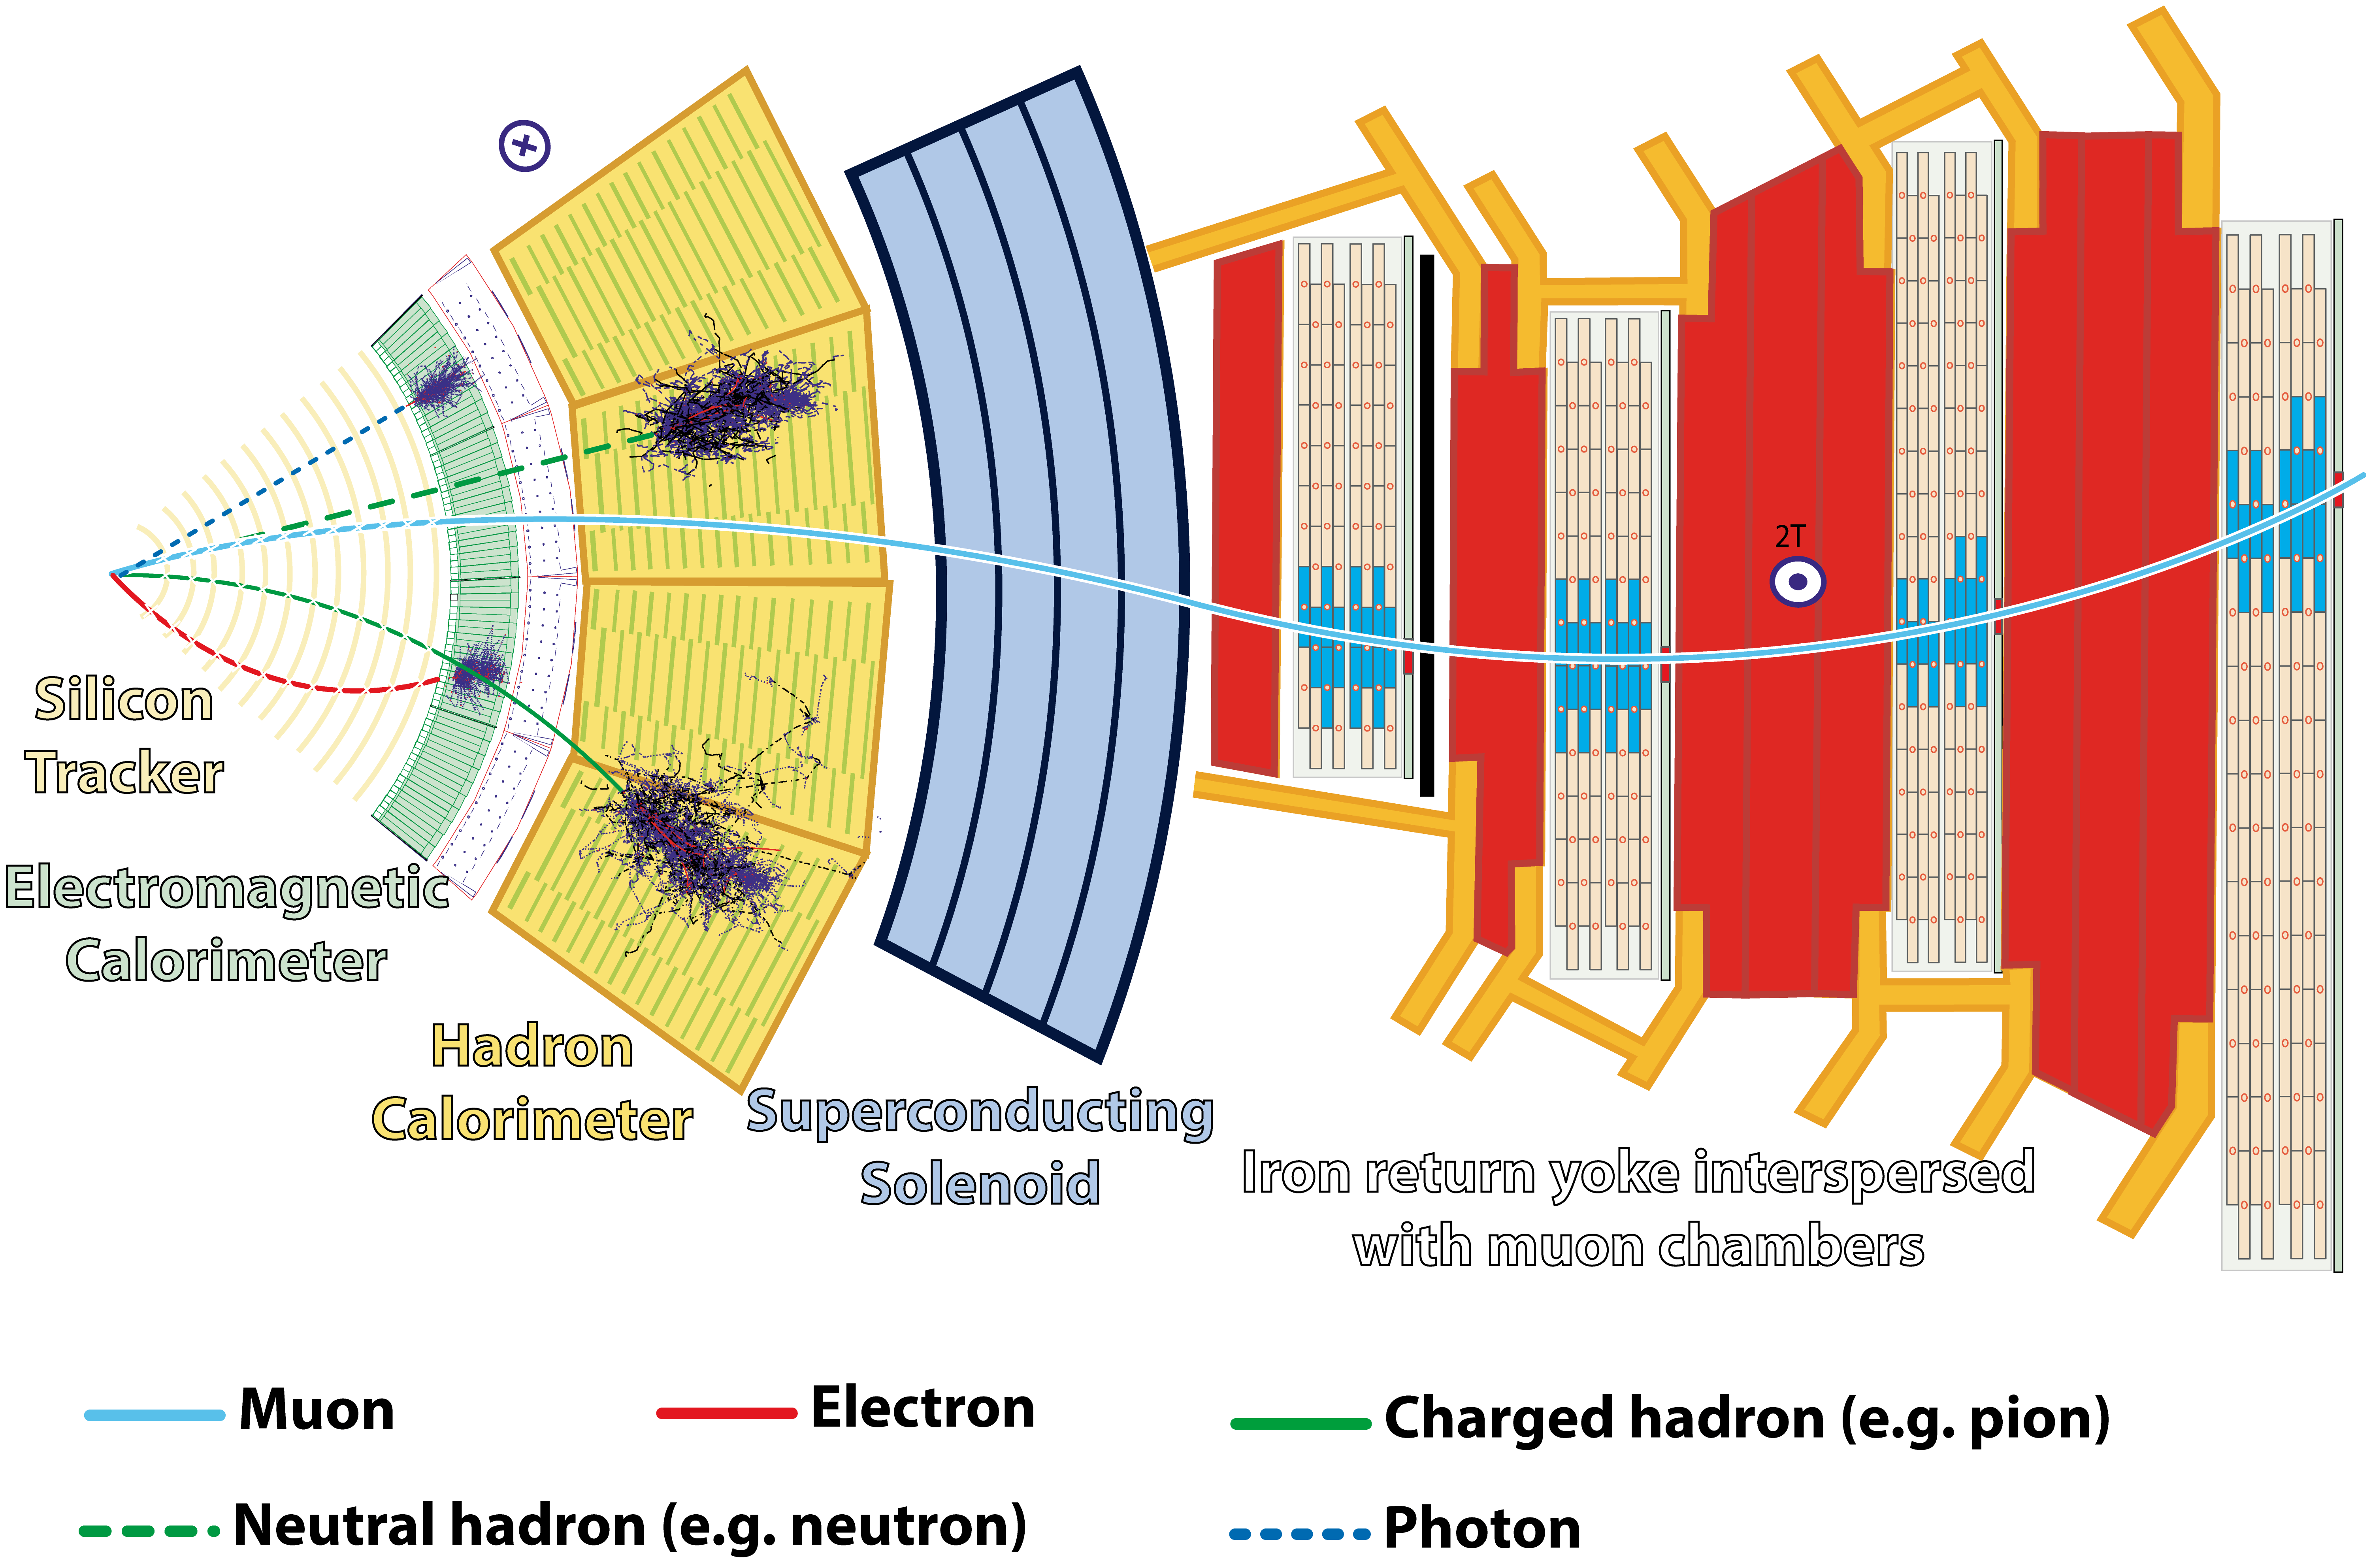
\includegraphics[width=\linewidth]{subfiles/imgs/CMSslice_whiteBackground.png}
    \caption{Shows the movement of different particles in the CMS detector \cite{Barney:2120661}.}
    \label{fig:particles_in_cms}
\end{figure}

The collision of charged particles in the LHC creates ionizing particles which over time will accumulate. The total ionizing dose (TID) expected after 10 years of operation has been simulated using FLUKA, a tool for monte carlo simulation of particle movement and their interactions. The expected dose decreases with distance from the collision point. A complete map of the expected TID for the detector can be seen in figure \ref{fig:tid_in_cms}.  

\begin{figure}[H]
    \centering
    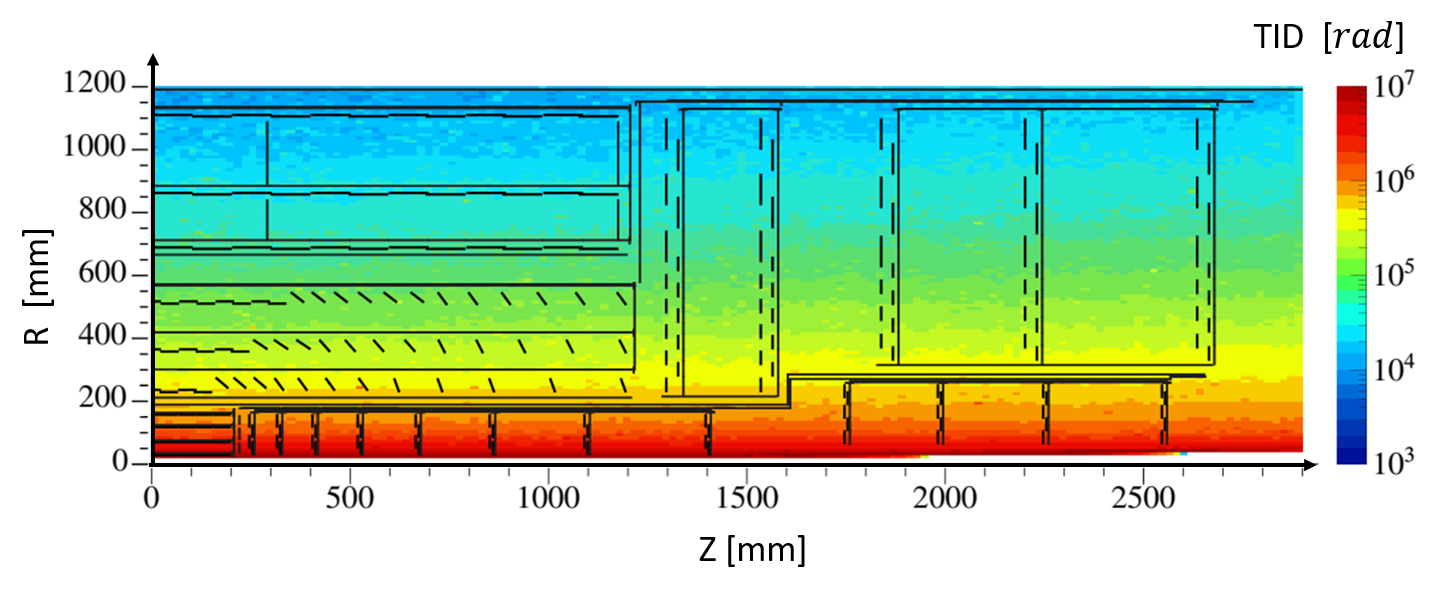
\includegraphics[width=\linewidth]{subfiles/imgs/CMS_RadiationLevels_2.png}
    \caption{Shows expected total ionizing dose in \si{Gy} during a 10-year operation period of the CMS. This is simulated using FLUKA. \cite{cms_tdr}}
    \label{fig:tid_in_cms}
\end{figure}

The ionizing dose and charged particles passing through electronics can alter their behavior and affect the output in unwanted ways. These effects will now be discussed in detail. 

\section{Radiation Effects on CMOS Electronics}
\label{rad_effect_cmos}
It is necessary to discuss and understand the effects of radiation on CMOS electronics due to the highly radioactive environment of the CERN accelerators. This understanding will lead to understanding the necessity and the methods for radiation hardening of the electronics. The radiation affects the CMOS in two distinguishable ways. In the form of cumulative damages and single-event effects (SEEs). 

\subsection{Cumulative Damages}
Cumulative damages can be split into two subcategories. The first is non-ionizing processes, which come in the form of displacement of atoms in the lattice structure of the transistor. These are called displacement damages and are of little concern to CMOS technologies due to the high amount of doping \cite{giulioThesis}. The second is damages induced by ionizing doses, i.e. TID effects. MOS transistors can accumulate charges in the gate oxide, which creates a voltage difference on the gate and leads to unwanted biasing. This effect is dominant when the gate oxide is thick as it can contain a larger charge compared to the voltage threshold of the gate. Therefore, this effect decreases with smaller technologies as the gate oxide becomes thinner. The smaller technologies are instead dominated by effects like shallow trench isolation (STI) effects, which come in the form of radiation-induced drain-to-source leakage current and radiation-induced narrow channel effects (RINCE) \cite{giulioThesis}. Radiation-induced drain-to-source leakage current is caused by the accumulation of positive charges in the STI, which opens parasitic channels between the source and drain. This leads to an increase in leakage current. Positive charges are far more likely to be trapped due to electrons moving fast enough to leave the STI, while electron holes do not. However, over time electrons are attracted and enough electrons can be attracted to invert this effect. Therefore, initially, an increase in leakage current is observed, but as TID increases this effect reaches a peak and begins to invert. Since only positive charges are initially trapped, this effect does not increase the leakage current of pMOS. Instead, it repels the holes of the doped silicon increasing its threshold voltage and decreasing current flow. It is clear that increasing the length of the channel, decreases this effect as more charge is to be trapped before a channel can be opened. Therefore this effect is significant in smaller technologies with short gate lengths. However, this effect can be mitigated by using enclosed layout transistors (ELT), where the channel does not face the STI. 
%In figure -- a traditional layout of a transistor and a ELT layout can be seen. \todo{add figure}   

The other effect is RINCE, which is also due to the trapped charges in the STI. As positive charges are trapped in the STI, an electric field is created. This electric field leads to a decrease in threshold voltage for nMOS transistors and an increase in threshold voltage for pMOS transistors. However, as the width of the channel decrease, this effect becomes more dominant as the number of trapped charges does not change. This leads to a proportionally larger electric field, which signifies a dependency on channel width for this effect. For nMOS transistors, this effect is limited, as negative charges become trapped at the interface leading to the two canceling out similar to the inversion seen in radiation-induced drain-to-source leakage current at higher TID. However, for pMOS the trapped charges at the interface are also positive, leading to RINCE only increasing in potency with an increase in TID. As this effect is also due to charges trapped in the STI, it can be mitigated by the use of ELT \cite{giulioThesis}. However, these ELTs do use significantly more area compared to traditional designs. 

\subsection{Single-Event Effects}
Single-Event effects can be split into two categories, permanent single-event effects, and single-event upsets (SEUs) (and transients (SETs)). A permanent single-event is the possible creation of parasitic transistor structures between two n-wells, i.e. between two transistors. This can potentially shorten VDD and ground, which can permanently damage the device. However, this effect is limited due to highly doped substrates and the use of STI between wells \cite{aleThesis}. 

SEUs and transients are soft errors and not destructive to the die. Instead, they corrupt the information stored in digital logic circuits by flipping bits. SEUs become possible when the collected fraction of the charge liberated by an ionizing particle is larger than the electric charge stored on a sensitive node \cite{aleThesis}. This critical charge scales with the gate area of the design. As the gate area decreases, the amount of stored charge representing a logical value of information decreases. In general, SEU sensitivity is increased by the scaling down of technology as node capacitance and the supply voltage are both scaled down as well \cite{aleThesis}. 

A SET is an event, where a static combinatorial circuit is upset by a charged particle, leading to a glitch in the circuit. The time duration of SET is determined by the injected charge and the driving strength of the cell. If the output of this combinatorial circuit is sampled during the transient, a register can enter a metastable state, which can propagate through causing fatal errors \cite{aleThesis}. 
%Displacement damage
%TID dmgs
%
%
%Single event effects
\section{Radiation-Tolerant Design}
\label{rt_design}
The goal of radiation-tolerant design is to limit the potential damage caused by radiation effects as described in section \ref{rad_effect_cmos}. Some of these effects can only be limited by a careful layout of the die or by the intrinsic properties of the chosen CMOS technology. However, SEUs can be reduced and mitigated by a combination of digital design. The methods for radiation hardening are usually dependent on redundancy either in space or in time. 

A common method is the use of triple module redundancy (TMR). In this method, each memory element (i.e. register) and the corresponding combinatorial logic are instantiated three times. The outputs from these three registers are then passed to a voting system, which outputs the majority vote. The voting system itself is also triplicated to minimize the chance of a SET upset. If a single voter is used and is sampled during the SET, an error will occur in the system, thus leading to a single-point of failure. To avoid the build-up of errors in the 3 different paths, the feedback loop of a state machine should be taken from the voted result. An example of a TMR radiation hardening can be seen in figure \ref{fig:spatial_triplication}.

\begin{figure}[H]
    \centering
    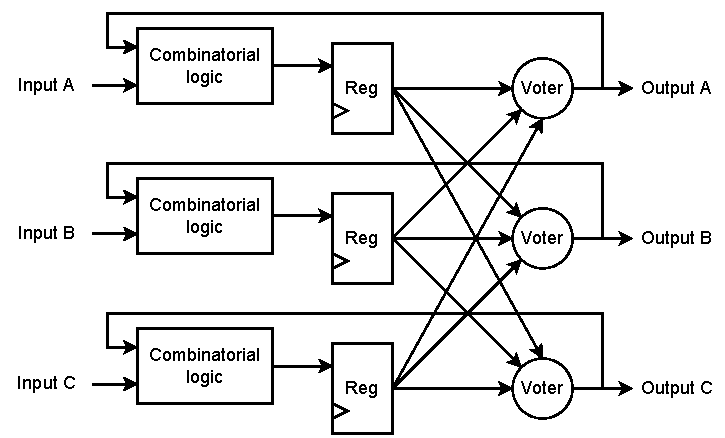
\includegraphics[width=0.7\linewidth]{subfiles/imgs/spacialTriplication.drawio (1).pdf}
    \caption{Shows a spatial radiation hardening technique using triple module redundancy.}
    \label{fig:spatial_triplication}
\end{figure}

This added redundancy would lose many of its radiation hardness benefits if the triplicated registers are placed close together on the chip die as this would increase the chance of an SEU happening on multiple registers from the same charged particle. Therefore the placement of these registers is restricted in the physical layout such that a minimum distance is enforced. 
%To reduce the chance of multiple errors from the same charged particle to a few percent, the distance has to be at least \SI{15}{\um} for \SI{65}{nm} technology \todo{kilde}. 
From this, it is clear that TMR increases radiation hardness by using space and power consumption (increased due to increase in hardware) as a trade-off. This increase in power and area is not cheap as the heat generated needs to be transported away from the detector and the space itself is limited inside the detector. Therefore to limit the disadvantages, the TMR is usually only done to the control path of a state machine. This is done as errors in the data path are limited in time, while an error in the control path can result in complete failure of the chip. At CERN, a tool has been developed for this method of radiation hardening named TMRG.

Another way of radiation hardening is the use of temporal spacing and is done by delaying the clock signal. The registers between combinatorial logic are triplicated, while the combinatorial logic itself, is not. Instead, the clock signal for each of the three registers is delayed, such that the SEU has a high statistical probability of having passed. This results in the SEU only affecting one register. It is then possible to use the same voting system as in TMR to achieve a corrected output. An example of this can be seen in figure \ref{fig:spatial_triplication}.

\begin{figure}[H]
    \centering
    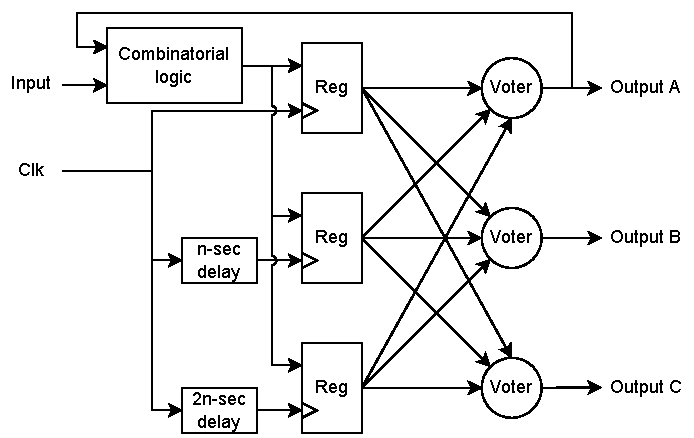
\includegraphics[width=0.7\linewidth]{subfiles/imgs/temporalTriplication.drawio.pdf}
    \caption{Shows a temporal radiation hardening technique where clock signals are delayed.}
    \label{fig:temporal_triplication}
\end{figure}

This method does not have the same minimum distance requirement as the TMR hardening technique as the registers sample at different timestamps. Instead, there is a temporal spacing requirement. 
%To lower the chance of affecting multiple registers to an acceptable level, the temporal spacing has been found to be at least \SI{200}{ps} \todo{kilde}. 
This method does not require a triplication of the  combinatorial logic and therefore saves on space and power consumption. However, it does make the timing analysis and closure difficult and this only gets more problematic as the frequency increases. 

Even though temporal radiation hardening has multiple advantages in the form of space and power consumption, the TMR is chosen due to its simpler implementation. This is due to the problematic nature of timing closure for the temporal radiation hardening, but also due to the existence of an already-developed tool for performing TMR. 


\section{Universal Verification Methodology}
\label{uvm}
The universal verification methodology (UVM) is an IEEE industry standard for the verification of design components \cite{uvmAccelleraScope}. It is developed by the Accellera group and its members. The goal is to create a modular, scalable and reusable generic verification environment. For these reasons, this methodology will be used for the verification of the SoC and its components. A short description of UVM will now be given.

UVM is based upon a hierarchy structure laid out by Accellera. This specifies guidelines for the creation of a verification environment and gives the support structure for this development. It does this by supplying a framework, for the designers to build on top of. This framework has the most general and essential features (Reporting, handshake mechanisms etc.), such that they do not need to be redeveloped for each project. This also ensures uniformity in testbench creation across many different work groups. The framework hierarchy is seen in figure \ref{fig:uvm_hierarchy} as it is laid out by Accellera \cite{uvmUserGuide}. Here the UVM agent can be expanded as it contains a sequencer, a driver, and a monitor. The expanded UVM agent can be seen in figure \ref{fig:uvm_agent}. Even though this is the recommended structure and should fit the most common use cases, the framework can be customized. 

\begin{figure}[H]
    \centering
    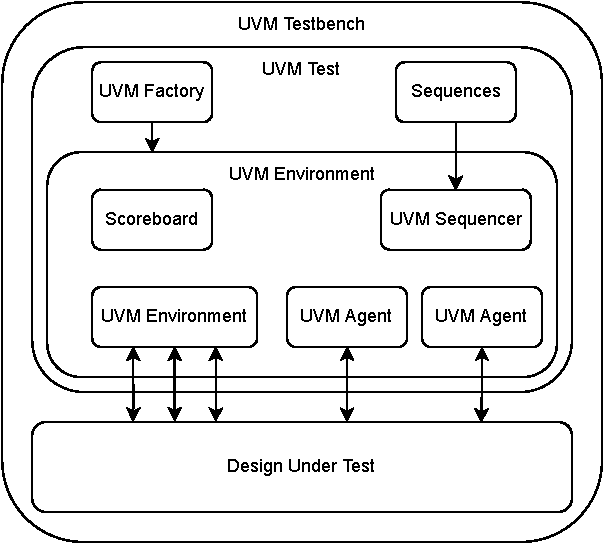
\includegraphics[width=0.6\linewidth]{subfiles/imgs/uvmHierarchy.drawio.pdf}
    \caption{Shows the complete hierarchy of the UVM structure laid out by Accellera.}
    \label{fig:uvm_hierarchy}
\end{figure}

\begin{figure}[H]
    \centering
    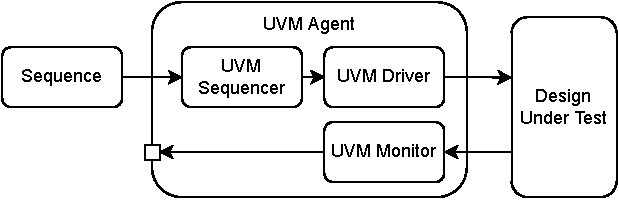
\includegraphics[width=0.6\linewidth]{subfiles/imgs/uvmAgentHierarchy.drawio.pdf}
    \caption{Shows the UVM components in a UVM agent and its connection to other components.}
    \label{fig:uvm_agent}
\end{figure}

The communication between components is based on transaction-level modeling (TLM) and UVM items. The items are designed to fit the specific device under test (DUT). It contains the information necessary to create stimuli to the DUT and updating scoreboard and reference module. The item is sent between components using TLM.

Each of the hierarchy levels has a base class associated with them. It is on top of these base classes that the project-relevant components will be built. Each of these classes and their functionality is described below \cite{uvmUserGuide}. 

\begin{itemize}
    \item \textbf{Testbench:} is the root class and container for all that needs to be simulated and tested. Typically this instantiates the DUT and the connections between the test and the DUT.
    \item \textbf{Test:} is the top-level UVM component. It has 3 main functions. To instantiate the test environment, configure the environment via a configuration database or factory overrides and apply stimulus to the DUT via the UVM sequences. This enables the designer to not have multiple instances of the same environment with different configurations for different test cases. Instead, the environment can be configured from this top-level UVM component to perform those test cases without repeating code.
    \item \textbf{Environment:} is a UVM component that instantiates and contains other reusable verification components such as agents, scoreboards, and other environments. It is also here the different components are connected and configured for default use. 
    \item \textbf{Scoreboard:} is the verification component that compares the DUT to an implemented reference module. The scoreboard does this by receiving UVM items from the DUT via the UVM agent using TLM ports. It can then use the reference module as a predictor and compare that to the DUT. 
    \item \textbf{Agent:} is a hierarchical component that contains other UVM components. These are typically a sequencer, a driver, and a monitor. The agent can either be active or inactive. An agent is active when it can drive stimuli to the DUT, which requires the use of a driver and sequencer. An inactive agent only contains a monitor.
    \begin{itemize}
        \item \textbf{Sequencer:} controls the flow of sequence items from the multiple sequences to the driver, i.e. queues different sequence items according to a set of given parameters.
        \item \textbf{Driver:} receives sequence items from the sequencer and converts them from transaction-level stimuli into pin-level stimuli for the DUT. For example, it can take a parallel data packet and transmit it via input pins to the DUT using a specified protocol. 
        \item \textbf{Monitor:} samples the DUT interface to convert data from pin-level stimuli into transaction-level stimuli. This data is then broadcast to the rest of the UVM testbench. The monitor can perform some levels of processing internally. For example, it can receive pin-level stimuli and decipher them according to a chosen protocol. So instead of broadcasting all pin-level activity, it first converts it into a specified UVM item and then broadcasts that using TLM.
    \end{itemize}
    \item \textbf{Sequence:} makes up the core stimuli of the verification plan. A sequence can be made of multiple data items which can be used to create the scenarios for testing the DUT extensively. The items are eventually sent to a sequencer which will then queue it and send it to the driver. Multiple sequences can be connected to the same sequencer. The randomization tools in UVM are commonly used in creating data items such that there is a higher chance of discovering bugs. A sequence is not part of the component hierarchy. A sequence can contain other sequences, called a parent or virtual sequence.  
\end{itemize}

A UVM environment can be developed either in SystemVerilog or SystemC, most commonly SystemVerilog. The SystemC variant is still under development but is in working condition. In this project, it has been chosen to use SystemC.

\section{Physical Implementation of Digital ICs}
\label{phys_imp_theory}
%%steps:
%%synthesis
%%mapping
%%syn_opt
%Implementation:
%floorplan
%place
%cts
%route
%checks
%drc
%lvs
%dynamic power analysis
%irdrop
%electromigration
%%different libraries
%threshold voltage
%%gate width
%antenna creation doing development

The PicoRV32 SoC will be implemented in a physical design. Therefore, a description of the steps from a digital design to a physical implementation will be given. The steps of physical implementation can in general be split into two categories: synthesis and implementation. Doing synthesis a Verilog design is converted from behavioral modeling into a gate-level description using only basic components supplied by a library. In the implementation, the gate-level description is converted into a physical implementation on a die with power distribution, a clock tree, and non-ideal components. Doing most steps, setup and hold conditions are checked for violations using different conditions. These are commonly referred to as corners. Corners are on-chip variations that alter the expected behavior of digital circuits and commonly include process, voltage, and temperature (PVT). The process variations are often summed and split into 3 categories slow (S), typical (T), and fast (F) for nMOS and pMOS transistors. 5 combinations (TT, SS, FF, SF, FS) of these corners can be evaluated to ensure that system works given variations and uncertainties. Setup and hold are tested in these corners, to ensure that the system behaves correctly even given on-chip variations. At CERN, radiation is included as an additional variation parameter. The TID effects are also evaluated in corners, using models developed at CERN for the behavior of chips doing radiation.

\subsection{Synthesis}
Synthesis is split into 3 steps: synthesis, mapping, and optimization. Doing synthesis a netlist is created from the supplied behavioral HDL model. For example, the always blocks in Verilog are converted into a basic set of components, e.g. flip-flop, AND-gate, NAND-gate. This step requires a list of constraints supplied by the designer. These constraints can be the clock period, output load capacitance, the maximum transition time of components, and setup/hold uncertainty on the clock. When this step is done, the Verilog code has been converted into a gate-level netlist that implements the same logic. 

The next step is mapping. Doing mapping a gate-level netlist is converted from using generic components to using components given by a library called standard cells. This library contains detailed descriptions of common cells in an implementation technology. The technology used in this project is \SI{28}{nm}. Many libraries exist for the same technology, but with different characteristics, e.g. track number, cell width, and gate length. The number of tracks refers to the height of each cell. The cell width is the number of which each cell width has to be a multiple of. Three libraries will be used as the default for physical implementation. The libraries will be 9 tracks high, a multiple of \SI{140}{\um} wide, and have a gate length of \SI{35}{nm}. The three libraries will have different threshold voltages. One will have a standard threshold, one will have an ultra-high threshold voltage and one will have a low-threshold voltage. The threshold voltage controls the voltage needed for the transistor to switch state. This is controlled by the amount of dopping on the source and drain of the transistor. However, lowering the threshold voltage increases the leakage current of the transistor. Different threshold voltages are therefore a trade-off between speed and power consumption. By including multiple libraries, the algorithms are given more options for optimization, such that speed requirements can be met by using low-threshold transistors or power consumption can be reduced by using ultra-high threshold transistors. The libraries contain a description of the physical layout of the cell, a timing model describing the delay from input to output, and noise models. After mapping the gate-level netlist described using generic components has been converted into a gate-level netlist with standard cell components from a specific library. 

After mapping, the last step of synthesis is optimization. Doing this step, different optimizations of the gate-level netlist are performed. This can be the removal of grounded circuits, removal of registers containing constants, or relocation of registers to reduce the amount needed. After all the steps have been completed estimates of certain parameters can be given for the digital design. This is things such as worst negative slack, power consumption, number of cells needed, and size of the complete design. 

\subsection{Implementation}
Implementation is the next step after synthesis. The implementation converts the gate-level netlist into a physical layout on a die. The steps of this are floorplan, place, clock tree synthesis, route, design finishing, and verification. 

Doing floorplanning, the die layout is designed. One of these variables is the die size. A rule of thumb is that the estimate at the end of synthesis should be 60\% of the final size. However, this does not account for the size of the power rings. These are chosen to be \SI{10}{\um} wide for both ground and VDD. This results in a spacing of \SI{25}{\um} of every side from the edge to the area in which standard cells can be placed (Extra space is needed to allow spacing between GND and VDD rings). Power rings are used to ensure a uniform distribution of power to all parts of the chip and to reduce the effect of IR drops. As the height of a standard cell is given by the library, the die is divided into rows with that height. The top and bottom of these rows can then be connected to the power by having wires going across from side to side. This creates a power mesh that supplies all the rows of standard cells with VDD and ground connections. On large designs, these lines can become long. Therefore, to minimize IR drop vertical and horizontal larger stripes are used to connect these tracks at multiple points. In the floorplanning, the height of the die is also given in metal tracks. For this project 9 metal (M1-M9) layers will be used. These do not have the same width. Instead, the top layer M1, has the highest routing width, M2 - M6 has the same width but is lower than M1, and M7-9 all decrease in routing width as the metal layer number goes up. M1 and M2 will be used for power distribution as these layers have the largest routing width and therefore the lowest resistance in the wires. M9 is used for the placement of standard cells and wiring. Usually, it is preferred to use the lower layers for wiring between standard cells as these signals do not draw significant current and the resistance is therefore not of concern. After this I/O ports are placed and if it is a top-level design, pads are also placed. 

The next step is placement. Here the standard cells are placed in the rows. This is with the goal of achieving minimal congestion and the best foundation for timing closure. This is typically done by keeping connecting cells close together. The tool also has to do the placement with the minimum distance between triplicated registers. 

The next step is clock tree synthesis. In this step, all the relevant components are connected to the clock signal. However, this is not a straightforward process. If the clock was just connected to all components without buffering, the clock edge would arrive at slightly different times depending on the placement of the component. Therefore the clock signal is continuously buffered to increase driving strength on long wires, but also to introduce delay in short wires, so that they arrive at nearly the same time, with the goal of not violating setup and hold time. This creates a tree-like structure. However, there is also a disadvantage to having all flip-flops latch at the same point in time, as this creates a large current spike which might cause IR drops and cause faults. Therefore if there is room in the setup and hold time, it is also an advantage to space out the latching in time, so that the current spike is limited. 

After clock tree synthesis, the next step is routing. This is done after clock tree synthesis because swapping these two steps would mean that the clock tree would have suboptimal wiring due to possible high congestion by routing. In the routing step all the connections specified by the gate-level netlist are established. If these wires are long, buffers are inserted to increase driving strength.

The design has now been placed and routed. Power and clock distribution have been established and in theory, the physical implementation process is finished. However, a few steps still remain to verify the design and ensure manufacturing is possible. For example, metal is filled into empty areas of the die. Without this sinkholes would be created and uneven metal layers would be laid on top, this would only get worse as more and more layers are added if nothing is routed or placed in that region. Therefore, metal is placed to create an even surface on which the metal can be laid. Next, design rule checks (DRC) and layout vs schematic (LVS) are performed. DRCs are manufacturing rules and safety protocols to ensure that the layout can actually be manufactured by the foundry. It can be simple things such as wire proximity checks, no short circuits, etc. However, there are also many complex rules. Things such as the area of a wire on a specific metal layer might be so big that it collects enough charge doing manufacturing that it destroys the connected component (Antenna effect). Another example is the concept of electromigration. When current is transported through a wire, it will slowly move material around. This effect increase with the amount of current. If this effect is too large, it means that some parts of the wire might become shallow and thereby increase resistance changing the behavior of a sensitive circuit. It can also short-circuit to a nearby wire if it gets too wide at places. It, therefore, checks if a wire is in danger of changing properties over a given lifetime. LVS checks whether the resulting layout at the end of the physical implementation is equivalent to the digital description from which it was derived.

With the physical implementation complete, we can generate an SDF file. This file contains all the propagation delays, clock arrivals, and such for the gate-level netlist. This can be used in combination with a testbench and the circuit can be verified to ensure that even given non-ideal clock signals and propagation delays, it still behaves as expected. Using this testbench and SDF file, a more accurate estimate of the switching activity of each transistor can be derived. This can be used in a dynamic power analysis to obtain a far more accurate estimation of power consumption. Before this, the tool just assumed that all transistor switches with a 20\% probability on each clock edge. This is the final step of physical implementation. All of this can then be collected in a set of files to establish a library for the implemented block. This can now be manufactured or used as a component in a larger design. 






\section{The PicoRV32: System on Chip}
\label{picorv_desc}
The goal of this project is to make a simple demonstrator SoC, with a CPU, memory blocks, and standardized interconnect bus with a basic set of peripherals. This demonstrator chip will then be used to test whether it is possible to create a radiation-tolerant SoC with a reasonable amount of area and power usage. Computing power is not of concern as its use case is targeted toward control and monitoring. RISC-V is an open-source instruction set architecture (ISA) that perfectly fits this application. Many different open-source SoC foundations have been considered and 3 stood out as candidates. Those are the Rocket Chip from UC Berkeley, the PicoSoC, and the Pulpissimo by ETH Zurich. The Rocket chip is a promising chip-building framework in Chisel. The PicoSoC is simple and written in pure Verilog, making it easier to understand. The Pulpissimo is made by ETH which has been collaborating with CERN before and therefore enables more direct communication with the designers. These three have been compared on their power and area usage during post-synthesis. The result of this can be seen in figure \ref{fig:CpuComparison}. Based on this comparison, the PicoSoC is chosen for the demonstrator chip.

\begin{figure}[H]
    \centering
    \begin{subfigure}[b]{0.49\textwidth}
        \centering
        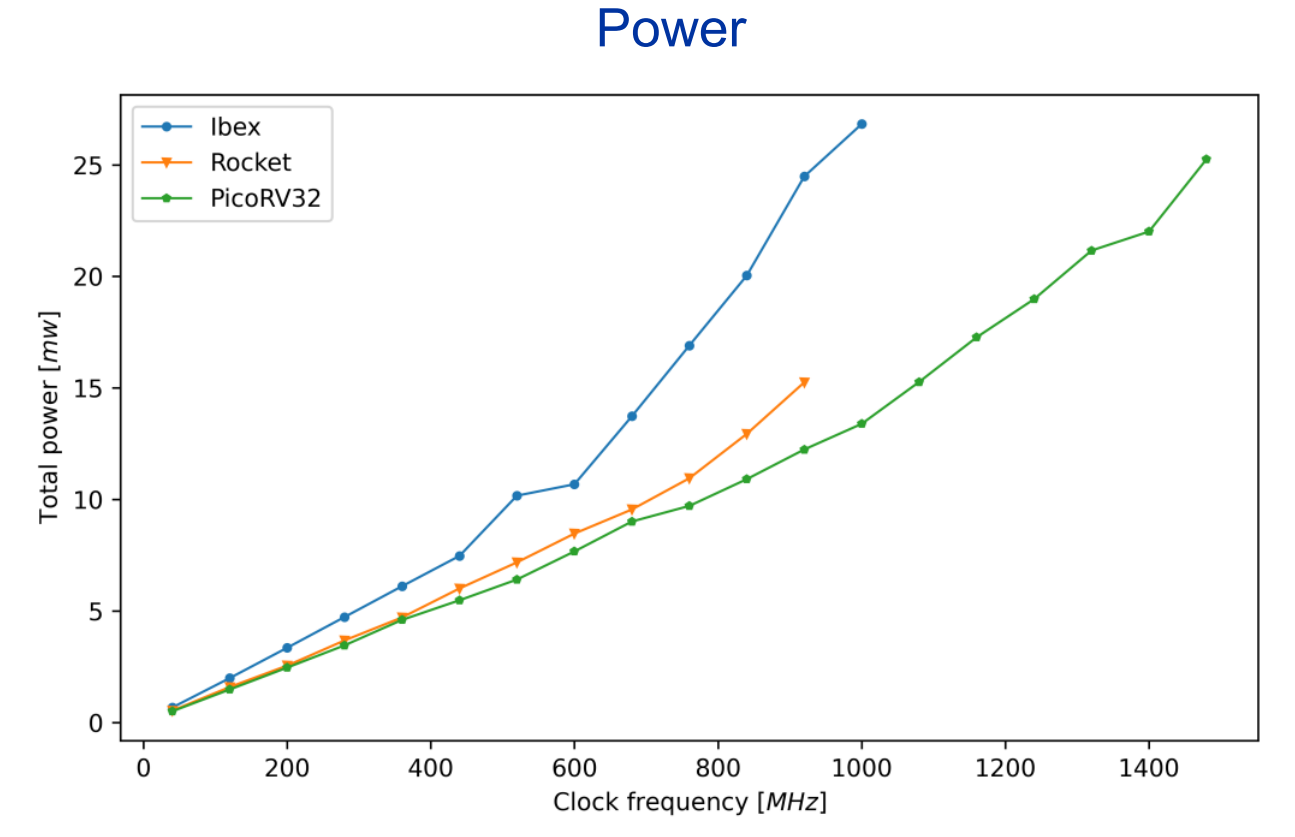
\includegraphics[width=\textwidth]{subfiles/imgs/cpuComparePower.png}
        \caption{}
        \label{fig:cpuComparePower}
    \end{subfigure}
    \hfill
    \begin{subfigure}[b]{0.49\textwidth}
        \centering
        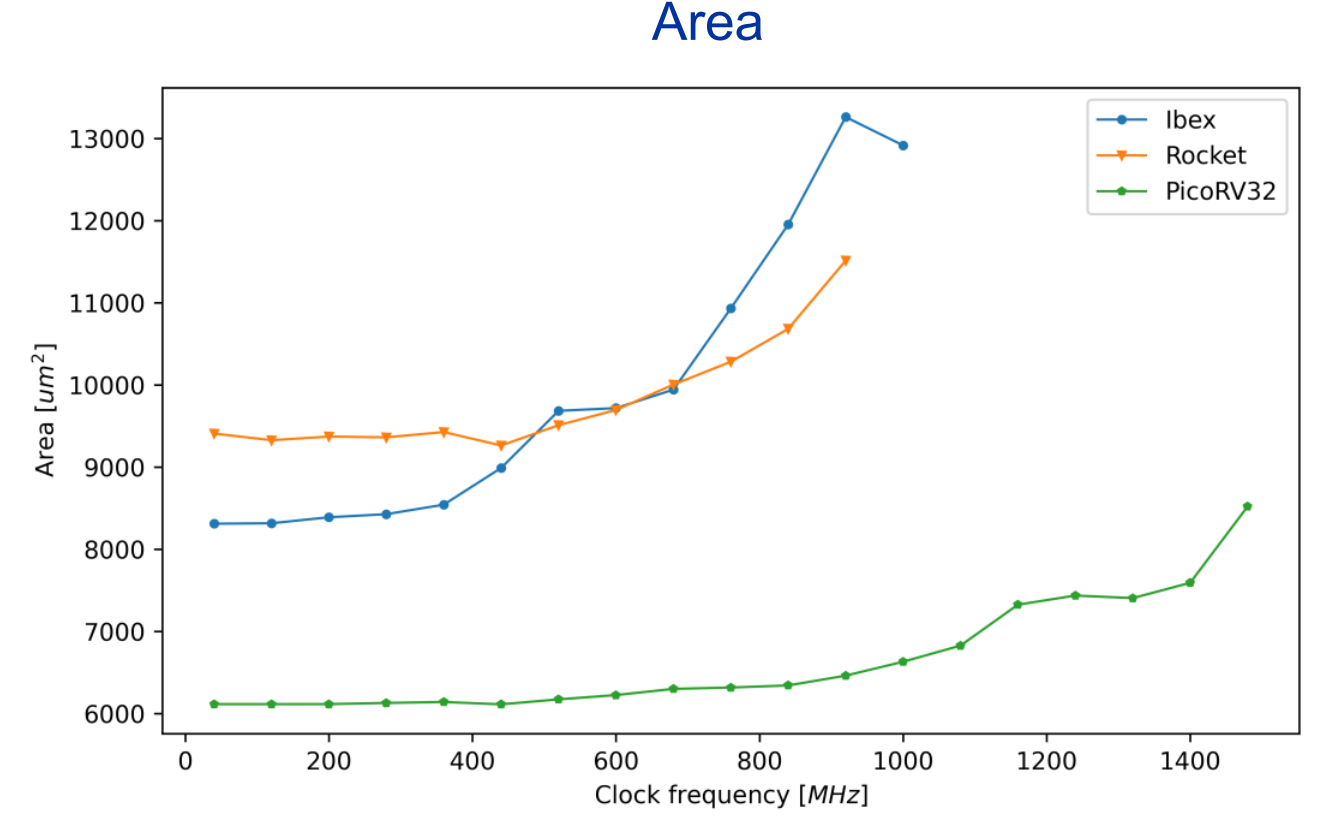
\includegraphics[width=\textwidth]{subfiles/imgs/cpuCompareArea.png}
        \caption{}
        \label{fig:cpuCompareArea}
    \end{subfigure}
    \hfill
    \caption{Shows the post-synthesis power and area comparison of an Ibex, Rocket, and PicoRV32 core.}
    \label{fig:CpuComparison}
\end{figure}

The PicoRV32 SoC is based upon the RISC-V open-source CPU: PicoRV32. This core is meant to be used as a size-optimized auxiliary CPU in an FPGA or ASIC design. It does not have high computational power, but it is small and simple. Due to its simplicity, it is also easier to debug and develop extra features. 

RISC-V is an open-source instruction set architecture (ISA). Its architecture is developed on Reduced Instruction Set Computer (RISC) principles. This is in contrast to the Complex Instruction Set Computer (CISC), to which the commonly known family of x86 ISAs belongs. The two design topologies differ because a CISC instruction often executes several lower-level instructions, while a RISC architecture does not. RISC-V employs a base set of the most needed instruction, while several extensions are available to expand the instruction set. The PicoRV32 is configurable \cite{picorv_nmi_if}. Its instruction base can be based on either RV32I (32-bit, base integer instruction set) or RV32E (32-bit, base integer embedded instruction set). The RV32I is capable of having two extensions added: multiplication (M) and the compressed instruction set (C). There is also an optional built-in interrupts controller. However, this is not based upon the RISC-V standard and is instead custom-built for the PicoRV32. This design choice was made because the RISC-V interrupt handle was extensive and comprehensive, so a simpler IRQ handling with less hardware overhead is available.

At the start of this project, several things were already implemented: The core, two buses, a bridge connecting the two busses, and a temporary memory block. A Native Memory Interface (NMI) connects the core and memory. The NMI is connected to a bridge that is connected to an Advanced Peripheral Bus (APB) interface. Peripherals will be connected to SoC using the APB interface. The state of the SoC at the beginning of this project is visualized in figure \ref{fig:PicoRV32SoC@beginning}.  

\begin{figure}[H]
    \centering
    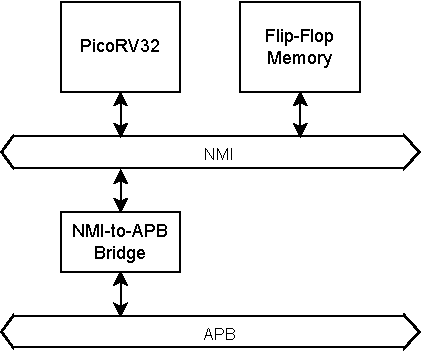
\includegraphics[width=0.5\linewidth]{subfiles/imgs/picorvSOCbeginning.drawio.pdf}
    \caption{Shows the state of the PicoRV32 SoC at the beginning of this project.}
    \label{fig:PicoRV32SoC@beginning}
\end{figure}

A detailed description of the two interfaces used on the buses is now given.

\subsection{Native Memory Interface}
\label{nmi_if}
The NMI is an interface defined by the PicoRV32 \cite{picorv_nmi_if}. It is a simple valid-ready interface bus. It requires five outputs from the PicoRV32 core and two outputs from the slave, which is receiving the transfer. These signals and their functions are described in table \ref{tab:nmi_sig}. This bus is only used to connect the most essential and critical blocks to the core, e.g., memory and bootloader. 


\begin{table}[H]
\centering
\caption{NMI signal descriptions}
\label{tab:nmi_sig}
\begin{tabular}{lll}
\hline
\textbf{Signal} \hspace{1cm} & \textbf{Source} \hspace{1.5cm} & \textbf{Description} \\ \hline
CLK & Clock source & Clock. The transfer is completed on the rising edge. \\ \hline
VALID & PicoRV32 core & \makecell[l]{Valid. The core uses the valid signal to initiate a \\ transfer. All core outputs are stable while valid is high.} \\ \hline
INSTR & PicoRV32 core & \makecell[l]{Instruction fetch. Used by the core to indicate if the \\ memory transfer is an instruction fetch}  \\ \hline
READY & Slave interface & \makecell[l]{Ready. Asserted by the slave when the read data is \\ available and used to acknowledge a write transfer.} \\ \hline
ADDR & PicoRV32 core & \makecell[l]{Address. The core supplies the address which is used by \\ the slave to read or write to the requested cell.} \\ \hline
WDATA & PicoRV32 core & \makecell[l]{Write data. If a write transfer is being performed, the \\ core supplies the data to be written using this bus} \\ \hline
WSTRB & PicoRV32 core & \makecell[l]{Write strobe. If the write strobe is 0, it indicates a read \\ transfer, while it being non-zero indicates a write \\ operation. The write strobe signal is used to write \\ specific bytes of the wdata. It is possible to write 32 bits, \\ the upper 16 bits, the lower 16 bits, or 8 bits.}  \\ \hline
RDATA & Slave interface &  \makecell[l]{Read data. In the case of read transfer, this is the data \\ read from the specified address. When rdata is available, \\ ready is asserted.} \\ \hline
\end{tabular}%

\end{table}

This bus is fully triplicated to achieve radiation hardening. This is decided due to it being critical infrastructure and also the length of this bus being limited since peripheral devices are not connected to this bus. 

\subsection{AMBA APB Interface}
\label{apb_if}
The APB is designed by ARM and is part of the Advanced Microcontroller Bus Architecture (AMBA) protocol family. This protocol has been chosen for the SoC since it is designed for minimal power consumption and reduced interface complexity \cite{apbReference}, which aligns with the goals of the project. The list of signals in the protocol can be seen in figure \ref{fig:apb_signals}.

\begin{figure}[H]
    \centering
    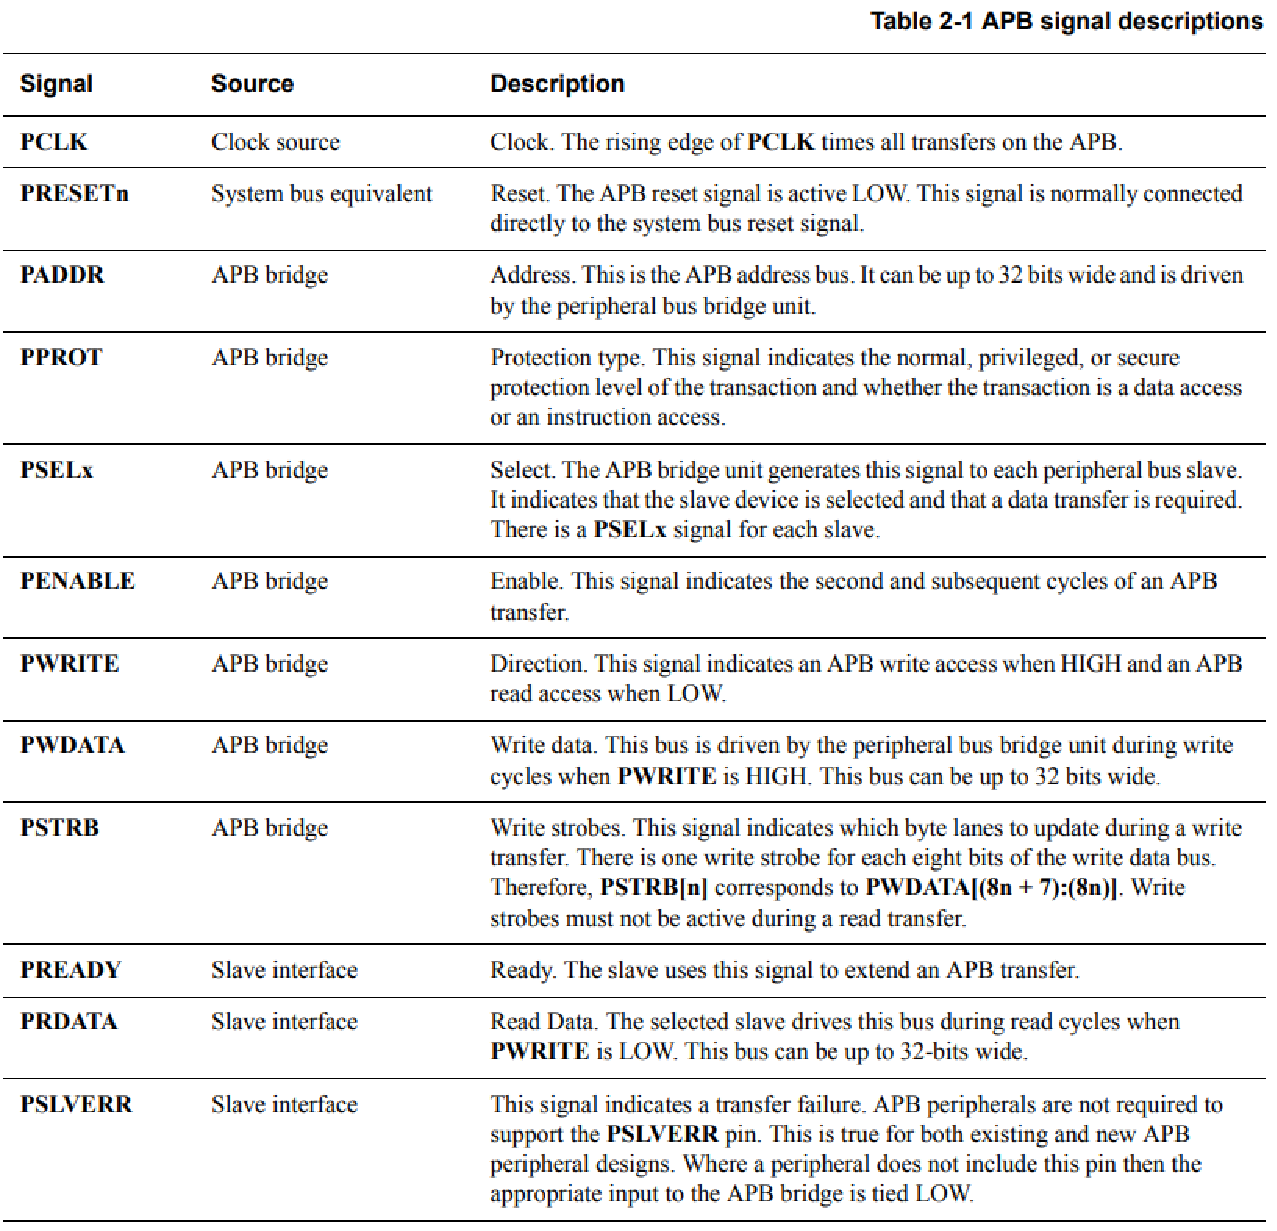
\includegraphics[width=\linewidth]{subfiles/imgs/IP_Blocks_Pics/apb_signals.pdf}
    \caption{Table of signals in the APB protocol (Courtesy of ARM \cite{apbReference}).}
    \label{fig:apb_signals}
\end{figure}

The protocol contains two individual buses for read and write operations. However, only one of these transfers can be executed at a time. The read and write transfer using the APB protocol with no wait cycles can be seen in figure \ref{apb_transfers_no_wait}.

\begin{figure}[H]
     \centering
     \begin{subfigure}[b]{0.49\textwidth}
         \centering
         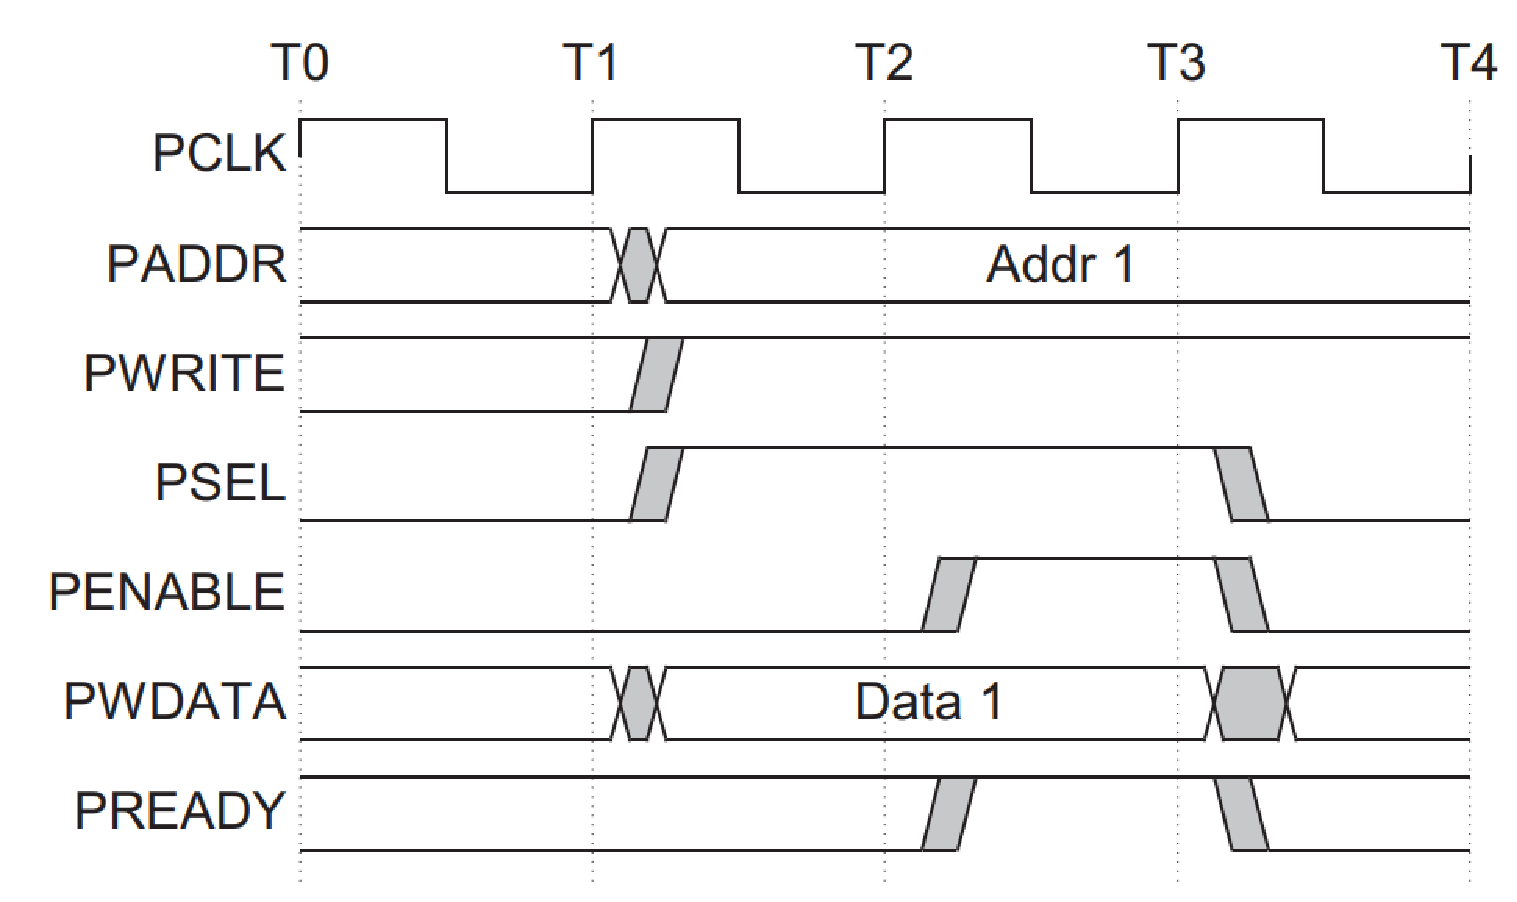
\includegraphics[width=\textwidth]{subfiles/imgs/IP_Blocks_Pics/apb_write_no_wait.pdf}
         \caption{Write transfer}
         \label{fig:apb_write_no_wait}
     \end{subfigure}
     \hfill
     \begin{subfigure}[b]{0.49\textwidth}
         \centering
         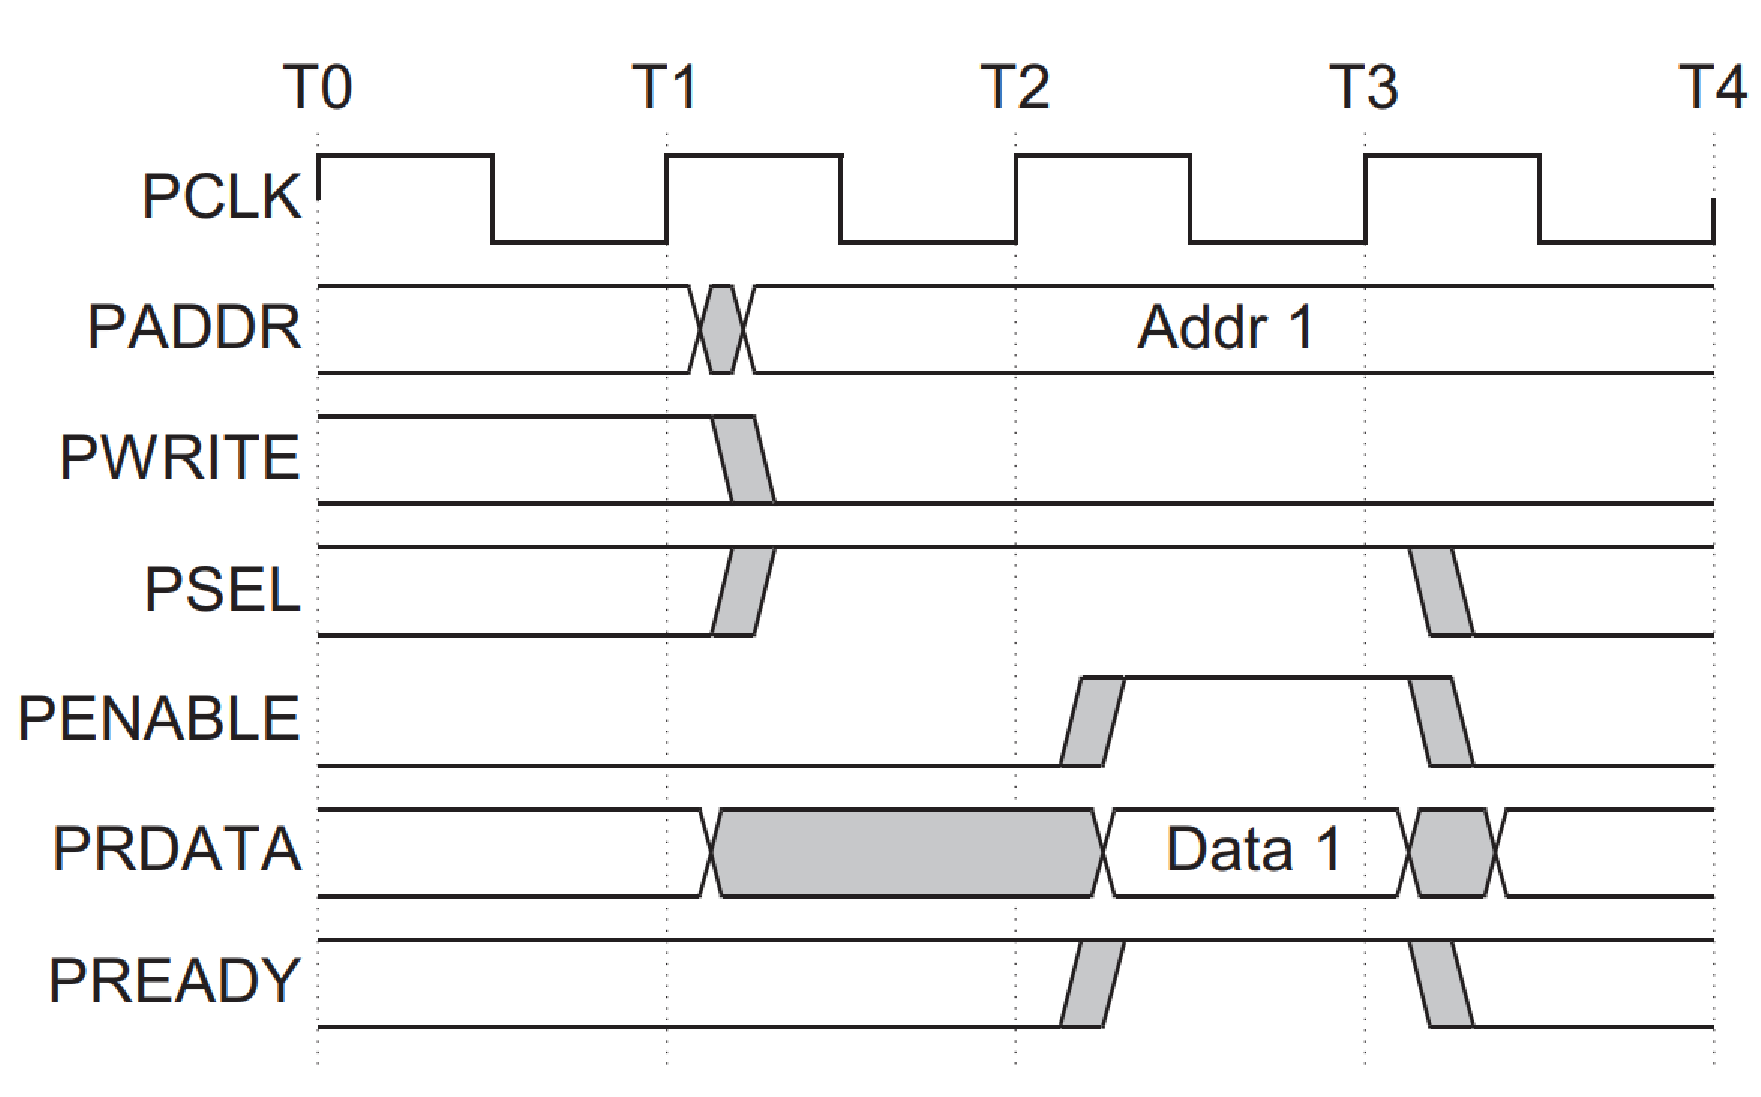
\includegraphics[width=\textwidth]{subfiles/imgs/IP_Blocks_Pics/apb_read_no_wait.pdf}
         \caption{Read transfer}
         \label{fig:apb_read_no_wait}
     \end{subfigure}
     \hfill
     \caption{Shows the basic transfers of the APB protocol with no wait cycles (Courtesy of ARM \cite{apbReference}).}
     \label{apb_transfers_no_wait}
\end{figure}

Wait cycles can be introduced if the slave does not assert the PREADY signal. However, the way the APB protocol is connected to the CPU will cause stalling of the entire CPU until the PREADY is asserted and the transfer is completed. A timeout could partially solve this by limiting the stalling period, but this does not fix the problem but only reduces it. Therefore it is chosen that the IP block as a general rule should always have PREADY asserted, as to ensure no stalling of the system. Instead in the case of a bad transfer due to no data available or similar situations, the PSLVERR signal is utilized and the IP block will then assert this signal to indicate that the transfer has failed. This introduces problems as this signal does not indicate why the transfer failed. However, it does remove the stalling. Therefore, this method is chosen. 

The APB bus will not be triplicated as this will connect all peripherals to the core and the length can therefore be quite significant, which will result in a larger area used and more complex routing. Instead, an encoding approach is used. Every byte of the bus is encoded using Hamming codes, which are capable of single error correction and double error detection. This approach uses the same logic developed later for radiation-tolerant memories. 









